\subsection{Iron Yoke Instrumentation}
%\writer{Valery Saveliev}{1}

Dedicated studies have been conducted at FNAL in the past years to optimize the layout of scintillator bars adapted to muon detection. Prototypes have been built and tested with muon beams~\cite{Denisov:2015jjl}. They are all based on long scintillator bars with signal collected by WLS fibers and readout by SiPMs at both extremities. The transverse resolution of $\approx$1cm required for the muon momentum measurement is defined by the bar widths of a few cm. The longitudinal position is measured from the time difference of the signals at both extremities and depends on the WLS configuration. The two options under consideration described in section 5.1.2 (Figure~\ref{fig:det:yoke}) have been tested: longitudinal resolutions of 5 to 10 cm are measured and found roughly independent of the longitudinal position of the muon within the bar (Figure~\ref{fig:det:Iron_proto}). 

More studies are ongoing to develop low cost SiPMs also adapted to the measurement of the tails of high energy jets (tail catcher function). 

The RPC option for the iron yoke instrumentation was not specifically studied but would directly benefit from the RPC developments of the SDHCAL hadronic calorimeter option (section~\ref{ild:sec:hcal:sdhcal}).   


\begin{figure}[t!]
\centering
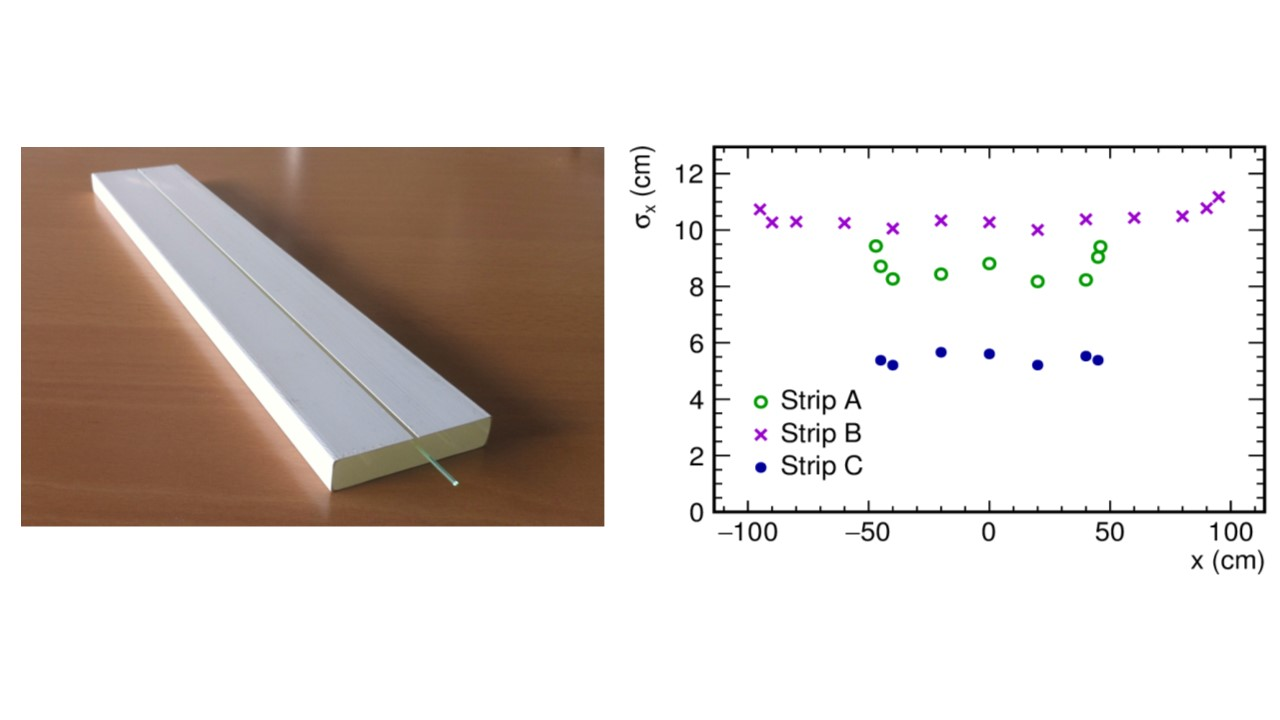
\includegraphics[width=1.0\hsize]{Detector/fig/Iron_proto.jpg}
\caption{Left: example of prototype scintillator bar built for the muon detector; right: longitudinal resolution on reconstructed muons as function of longitudinal coordinate: strip A and B as shown on the left of the figure with lengths of 1 and 2\,m respectively, strip C of 1\,m length with WLS fibers positioned on the small edge of the strip.}
\label{fig:det:Iron_proto}
\end{figure}
\hfill
